% Matteo Kumar - Leonard Schatt
% Fortgeschrittenes Physikalisches Praktikum
% 4.Kapitel Versuchsauswertung


For the ensemble measurements the fourteen samples of rods of different lengths and widths were measured with unpolarized light and light of \ang{0} and \ang{90} polarization each. The measured spectra $I_m$ were corrected using a reference spectrum $I_r$ taken without a sample for each of the three polarization setups. The corrected spectra $I_c$ were thus calculated as
\begin{equation}
    I_c = \frac{I_m}{I_r}.
\end{equation}
Although a dark spectrum $I_d$ was taken as well, it was not used for this evaluation, since $I_m$, $I_r$ and $I_d$ converged to the same intensities for increasing wavelengths and therefore created singularities when subtracting $I_d$ from both $I_m$ and $I_r$. This could be done since the values for $I_d$ were constant and small for the relevant parts of the wavelength scale. The corrected spectra can be seen in fig.~\ref{fig:unpol}, \ref{fig:pol0} and \ref{fig:pol90}. Using a gaussian function the wavelength for the maximum intensity $\lambda_{max}$ was calculated. All values can be found in tab.~\ref{tab:lamMaxUn},~\ref{tab:lamMax0} and \ref{tab:lamMax90}.

\begin{figure}
    \centering
    \begin{subfigure}{\textwidth}
        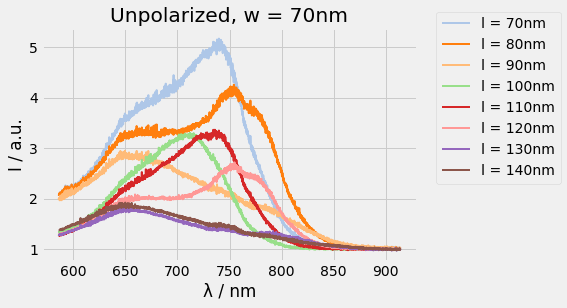
\includegraphics[width=\textwidth]{Bilder/Auswertung/SpektrumUnpol70.png}
        \caption{ }
        \label{fig:u70}
    \end{subfigure}
    \hfill
    \begin{subfigure}{\textwidth}
        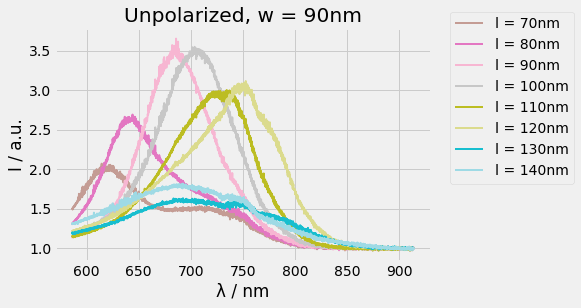
\includegraphics[width=\textwidth]{Bilder/Auswertung/SpektrumUnpol90.png}
        \caption{ }
        \label{fig:u90}
    \end{subfigure}
    \caption{The corrected spectra of the samples using unpolarized light are shown. While the rodlength varied throughput the samples, the rodwith of \SI{70}{\nano\meter} was fixed in (a) and one of \SI{90}{\nano\meter} in (b).}
    \label{fig:unpol}
\end{figure}

\begin{figure}
    \centering
    \begin{subfigure}{\textwidth}
        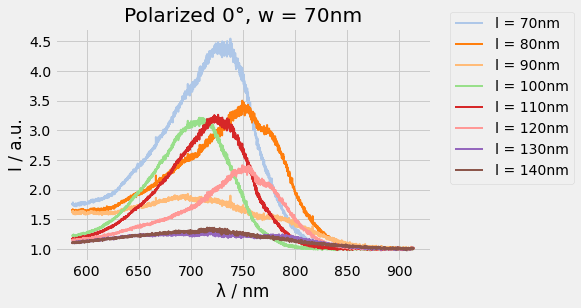
\includegraphics[width=\textwidth]{Bilder/Auswertung/SpektrumPol070.png}
        \caption{ }
        \label{fig:0-70}
    \end{subfigure}
    \hfill
    \begin{subfigure}{\textwidth}
        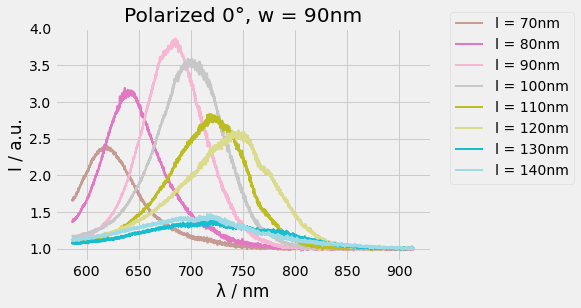
\includegraphics[width=\textwidth]{Bilder/Auswertung/SpektrumPol090.png}
        \caption{ }
        \label{fig:0-90}
    \end{subfigure}
    \caption{The corrected spectra of the samples using polarized light of \ang{0} are shown. While the rodlength varied throughput the samples, the rodwith of \SI{70}{\nano\meter} was fixed in (a) and one of \SI{90}{\nano\meter} in (b).}
    \label{fig:pol0}
\end{figure}

\begin{figure}
    \centering
    \begin{subfigure}{\textwidth}
        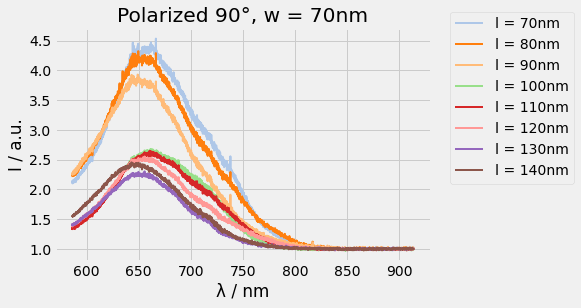
\includegraphics[width=\textwidth]{Bilder/Auswertung/SpektrumPol9070.png}
        \caption{ }
        \label{fig:90-70}
    \end{subfigure}
    \hfill
    \begin{subfigure}{\textwidth}
        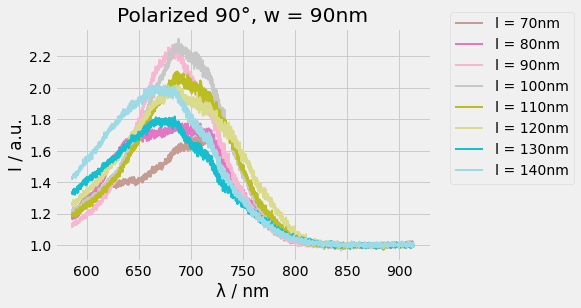
\includegraphics[width=\textwidth]{Bilder/Auswertung/SpektrumPol9090.png}
        \caption{ }
        \label{fig:90-90}
    \end{subfigure}
    \caption{The corrected spectra of the samples using polarized light of \ang{90} are shown. While the rodlength varied throughput the samples, the rodwith of \SI{70}{\nano\meter} was fixed in (a) and one of \SI{90}{\nano\meter} in (b).}
    \label{fig:pol90}
\end{figure}

\begin{table}
    \centering
    \begin{tabular}{c|cc}
        \toprule
        $l$ / \si{\nano\meter} &   $\lambda_{max,unpol,w=\SI{70}{\nano\meter}}$ / \si{\nano\meter}& $\lambda_{max,unpol,w=\SI{90}{\nano\meter}}$ / \si{\nano\meter}\\
        \midrule
        70  &  $708.2 \pm 0.4$&  $602.2 \pm 2.8$\\
        80  &  $741.5 \pm 1.0$&  $653.8 \pm 0.4$\\
        90  &  $669.6 \pm 0.3$&  $687.98 \pm 0.08$\\
        100 &  $696.44 \pm 0.18$&  $703.84 \pm 0.10$\\
        110 &  $712.5 \pm 0.3$&  $719.30 \pm 0.16$\\
        120 &  $757.6 \pm 1.4$&  $743.9 \pm 0.4$\\
        130 &  $668.5 \pm 0.4$&  $707.67 \pm 0.15$\\
        140 &  $664.8 \pm 0.3$&  $690.03 \pm 0.12$\\
        \bottomrule
    \end{tabular}
    \caption{Values of the wavelength of the maximum intensity of the spectra in fig.~\ref{fig:unpol}. All values were calculated from a fit using a gaussian function. The error represents the fitting error.}
    \label{tab:lamMaxUn}
\end{table}

\begin{table}
    \centering
    \begin{tabular}{c|cc}
        \toprule
        $l$ / \si{\nano\meter} &   $\lambda_{max,\ang{0},w=\SI{70}{\nano\meter}}$ / \si{\nano\meter}& $\lambda_{max,\ang{0},w=\SI{90}{\nano\meter}}$ / \si{\nano\meter}\\
        \midrule
        70 &  $715.1 \pm 0.3$&  $619.92\pm 0.15$\\
        80 &  $752.4 \pm 0.9$&  $642.88\pm 0.11$\\
        90  &  $688.1\pm 0.3$&  $683.02\pm 0.05$\\
        100 &  $700.21\pm 0.16$&  $699.07\pm 0.09$\\
        110 &  $716.48\pm 0.19$&  $716.39\pm 0.12$\\
        120 &  $751.4\pm 0.6$&  $736.7\pm 0.2$\\
        130 &  $709.5\pm 0.4$&  $715.3\pm 0.2$\\
        140 &  $705.8\pm 0.2$&  $699.33\pm 0.17$\\
        \bottomrule
    \end{tabular}
    \caption{Values of the wavelength of the maximum intensity of the spectra in fig.~ \ref{fig:pol0}. All values were calculated from a fit using a gaussian function. The error represents the fitting error.}
    \label{tab:lamMax0}
\end{table}

\begin{table}
    \centering
    \begin{tabular}{c|cc}
        \toprule
        $l$ / \si{\nano\meter} & $\lambda_{max,\ang{90},w=\SI{70}{\nano\meter}}$ / \si{\nano\meter}& $\lambda_{max,\ang{90},w=\SI{90}{\nano\meter}}$ / \si{\nano\meter}\\
        \midrule
        70  &  $664.06\pm 0.11$&  $687.18\pm 0.4$\\
        80  &  $659.13\pm 0.12$&  $678.41\pm 0.17$\\
        90  &  $651.89\pm 0.08$&  $684.50\pm 07$\\
        100 &  $668.10\pm 0.08$&  $690.46\pm 0.13$\\
        110 &  $668.06\pm 0.11$&  $691.38\pm 0.11$\\
        120 &  $660.99\pm 0.13$&  $688.20\pm 0.10$\\
        130 &  $653.20\pm 0.07$&   $668.06\pm 0.11$\\
        140 &  $649.43\pm 0.06$&  $664.28\pm 0.09$\\
        \bottomrule
    \end{tabular}
    \caption{Values of the wavelength of the maximum intensity of the spectra in fig.~\ref{fig:pol90}. All values were calculated from a fit using a gaussian function. The error represents the fitting error.}
    \label{tab:lamMax90}
\end{table}


    
As well in fig.~\ref{fig:pol90} as in tab.~\ref{tab:lamMax90} can be seen that in the case of a polarization of \ang{90} the wavelength at the maximum of the intensity spectra does not shift with a varying rodlength. This corresponds to the literature which lets us expect no shifting of the maxima for the transversal modes~\cite{LehrstuhlExperimentalphysikIII.2023}. On the other hand, for the longitudinal modes (i.e.~a polarization of \ang{0}), a shift of the maximum can be observed in fig.~\ref{fig:pol0} and in tab.~\ref{tab:lamMax0}, both. The unpolarized spectra should show characteristica of transversal and longitudinal modes, as both are excited. This is the case here, as can be seen especially for $w$ = \SI{90}{\nano\meter} (and e.g.~$l$ = \SI{80}{\nano\meter}). Hereby can be seen, that the peaks for the transversal modes are smaller as the ones of the longitudinal modes (except the cases for $l<w$ for obvious reasons). Further, the calculated maxima for \ang{0} polarization match the calculated maxima for the measurements using unpolarized light. This is a further confirmation of our measurement since \ang{0} polarized light should be part of unpolarized light. \par 
As stated above, the maximum wavelength $\lambda_{max}$ depends on the rodlength when using \ang{0} polarized light. We expect to find a linear correlation, as the literature states 
\begin{equation}
    m \lambda = 2n_{eff}(L(m)+\Delta L),
\end{equation}
with the effective refractive index of the plasmon $n_{eff}$ and its resonator length $L(m)+\Delta L$~\cite{LehrstuhlExperimentalphysikIII.2023}. Using the ground mode ($m=1$) one gets 
\begin{equation}
    \lambda (L) = 2n_{eff}L + 2n_{eff}\Delta L.
\end{equation}
Therefore, a fit was made based on a linear function. This is illustrated in fig.~\ref{fig:rodlength}. Hereby, for $w =$ \SI{70}{\nano\meter} and $w =$ \SI{90}{\nano\meter} the datapoints of $l =$ \SI{130}{\nano\meter} and $l =$ \SI{140}{\nano\meter} as well as the points of $l =$ \SI{70}{\nano\meter} and $l =$ \SI{80}{\nano\meter} just in the case for $w =$ \SI{70}{\nano\meter} were omitted, as they were far off the expectations. In the cases of the former, the intensity curves were very broad (see fig.~\ref{fig:0-70} and~\ref{fig:0-90}) and therefore the maxima may not be calculated as precise as needed.

\begin{figure}
    \centering
    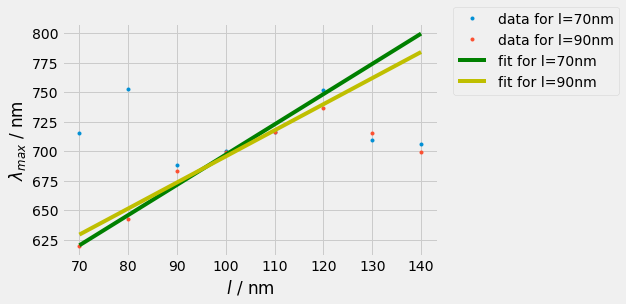
\includegraphics[width=\textwidth]{Bilder/Auswertung/fitRods.png}
    \caption{The maximum wavelength depends linear on the rodlength as the fitted lines show.}
    \label{fig:rodlength}
\end{figure}

Both fitted lines show similar properties. This is up to our expectations since $n_{eff}$ and $\Delta L$ should not depend on the rodlength. Evaluating the slope and y-axis intersection and then averaging over both measurements one yields \par 

\centerline{\boxed{n_{eff} = \num{1.2 \pm 0.3} \qquad \Delta L = \SI{190 \pm 28}{\nano\meter}.}}

$n_{eff}$ seems resonable since a value of $n_{eff} =$1.4 can be used to describe a particle at a water/air interface~\cite{LehrstuhlExperimentalphysikIII.2023}. The values for $\Delta L$ are quite high comparing them with the actual lengths of the rods. That means that the length of the resonator can be over trice the length of the rods themself in our measurements. However, this aligns with the literature, which states, that the plasmonic electrical field outside the plasmon does not exceed \SI{100}{\nano\meter} which would correspond to $\frac{\Delta L}{2}$~\cite{Chen.2013}.